\section{Function as a Service -- FaaS}
\begin{itemize}
	\item extension of \textbf{Platform-as-a-Service} model, provides \textbf{platform for serverless computing}.
	\item \textbf{Serverless Computing}: develop, run, and manage application \textbf{functionalities} \textbf{without worrying about the underlying infrastructure/scaling} (physical/virtual servers).
	\begin{itemize}
		\item FaaS: \textbf{event-driven} computing, functions are \textbf{triggered} by events/http-requests
		\item Backend-as-a-Service(BaaS): third-party API services that replace core subsets of functionality in application.
	\end{itemize}
	\item Advantages:
	\begin{itemize}
		\item \textbf{concentration on development of application} instead of deployment/allocation/scaling of resources.
		\item no provisioning of servers, automatic scaling(no autoscaling policies)
		\item cost reduction. \textbf{Pay per function invocation}. (Microservice: one instance when service is not used will be paid.)
	\end{itemize}
	Disadvantages: 
	\begin{itemize}
		\item focuses on \textbf{stateless functions}
		\item unsuitable for heavy workloads $\rightarrow$ too many invocations, expensive
		\item limited security: shared VMs, no control over network
		\item vendor lock-in
	\end{itemize}
	\item When to FaaS: 
	\begin{itemize}
		\item easily \textbf{decomposable} functions
		\item highly-\textbf{variable demand} -- autoscaling being taken cared.
		\item \textbf{low/medium frequency function triggering}, overhead in running instance is high (pricing)
		\item need for tight integration to cloud events
	\end{itemize}
	
	
	\item Use-case: Amazon Lambda, OpenWhisk(open source)
	
\end{itemize}

\subsection{AWS Lambda}
\begin{itemize}
	\item lambda functions: anonymous functions, often used as \textbf{arguments} being passed to higher-order functions or as result of a higher-order function.
	\item event sources:
	\begin{itemize}
		\item data stores(insert/delete in dymnamo DB, image upload on S3),
		\item endpoints(API requests, IoT measurements)
		\item development and management tools(CloudWatch monitoring results)
		\item event/message services
	\end{itemize}
	\item execution model: synchronous, asynchronous(event queue), stream-based
	\item Pricing: \#requests, compute time
	\item Architecture:
	
	\begin{figure}[H]
		\centering
		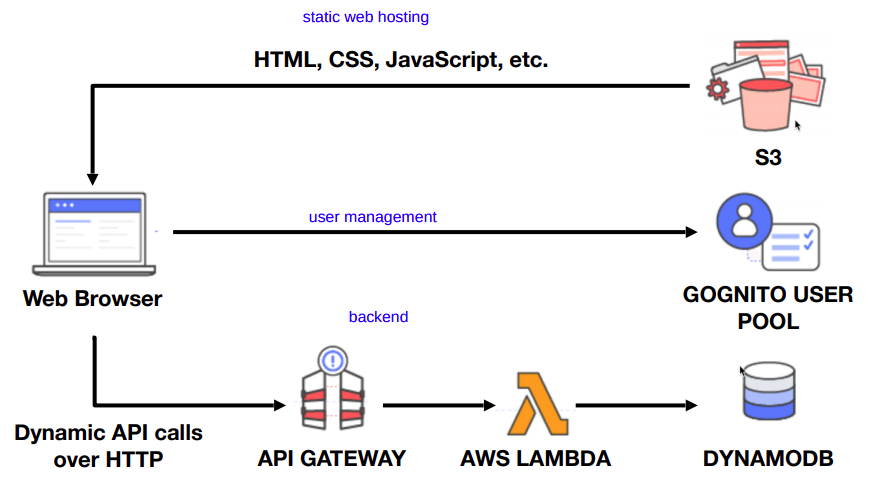
\includegraphics[width=0.8\textwidth]{lambda.png}
	\end{figure}
	\begin{itemize}
		\item static web hosting in S3: \textbf{static web content} for user interface are \textbf{stored into a bucket and registered} in S3 $\rightarrow$ gets a public URL
		\item \textbf{user management} with Cognito
		\item serverless service backend: \textbf{handles requests}
		\begin{itemize}
			\item requests from browser --> API Gateway invokes lambda function --> Amazon lambda function implementation --> access/request in Dynamo DB in the cloud
			\item Dynamo DB: create table, Identity and Access Management role for lambda function (permission to write into Dynamo DB using lambda function)
		\end{itemize}
	\end{itemize}
\end{itemize}


\subsection{OpenWhisk}
\begin{itemize}
	\item open source FaaS platform
	\item Concept: \textbf{event sources trigger action codes}
	\begin{itemize}
		\item trigger: named channels for classes or kinds of events sent from Event Sources
		\item rules: associate one trigger with one action. After an association is created, each time a trigger event is fired, the action is invoked.
		\item action invocation: 
		\begin{itemize}
			\item blocking: calls action, wait until it's executed, return value delivered
			\item non-blocking: action trigger is recognized, returns immediately(might be no value if not available) without waiting for action execution 
		\end{itemize}
		\item action chaining
	\end{itemize}
	\begin{figure}[H]
		\centering
		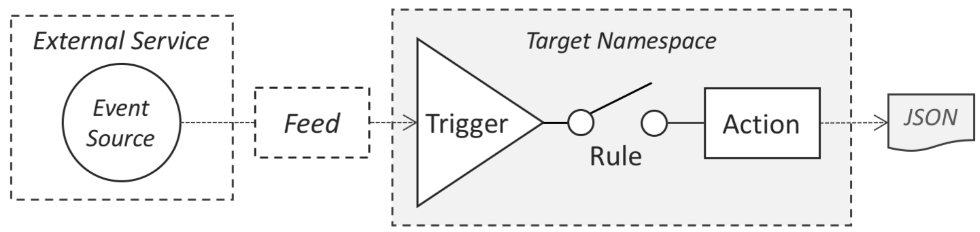
\includegraphics[width=0.8\textwidth]{openwhisk.png}
	\end{figure}
	\item Architecture \& Process: 
	\begin{itemize}
		\item \textbf{entering the system -- nginx}: front-end, a HTTP user API into the system. \textbf{Requests send into system}.		
		\item \textbf{entering the system -- controller}: \textbf{user authentication and authorization}(gets from \textbf{CouchDB}). when succeeds, translates user \textbf{requests into an invocation of actions}.
		\item \textbf{getting the action -- CouchDB}: actions (codes + default parameters) are loaded into CouchDB. It merges with the user request parameters.
		\item \textbf{choosing action invoker -- load balancer(controller)}: checks available executors(\textbf{invokers})
		\item \textbf{queue -- Kafka}: handles two issues: losing invocation(system crashes) and waiting(heavy workload). Controller publishes \textbf{message}(action to invoke, user parameters, allocated invoker) to Kafka. User gets activationID. \textbf{Asynchronous execution}.
		\item \textbf{invoking codes -- invoker}: invokes actions. Execution of actions are isolated \textbf{inside a container}(Docker).  
		\item \textbf{storing the results -- CouchDB}: action results saved as \textbf{JSON object into CouchDB}
		\item \textbf{getting the result -- nginx}: get result using activationID. 
	\end{itemize}
	\begin{figure}[H]
		\centering
		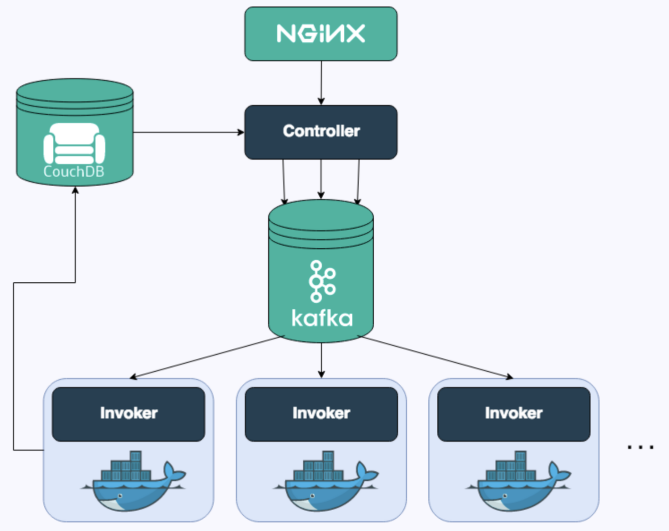
\includegraphics[width=0.7\textwidth]{openwhiskarchi.png}
	\end{figure}




	\item Optimization: \textbf{reduce cold start time} -- time to prepare container to start
	\begin{itemize}
		\item \textbf{cold container}: container has to be \textbf{created from scratch} $\rightarrow$ longest cold start time.
		\item \textbf{pre-warmed container}: pre-allocated container with \textbf{initialized runtime environment}(eg: nodejs). It needs to initialize and run the function.   
		\item \textbf{warm container}: container with \textbf{initialized function and runtime environment}. It can directly \textbf{rerun same subsequent} function invocations. 
		\item \textbf{hot container}: container with \textbf{running function and runtime environment}. Within the grace-period, it \textbf{executes same subsequent} functions invocations. 
	\end{itemize}
	
	
	\item function composition(chaining): 
	\begin{itemize}
		\item target: small, simple, stateless functions
		\item approaches:
		\begin{itemize}
			\item client side: calls one function that executes both
			\item server side: double billing problem
			\item event-driven: first function triggers second
			\item \textbf{premitive sequence}: define a sequence in command-line.
			
			$\rightarrow$ no special code required, no knowledge required about function relationship, no double costs.
		\end{itemize}
	\end{itemize}
	
\end{itemize}


